\documentclass[12pt,twoside]{report}
\usepackage[utf8]{inputenc}
\usepackage{titlesec, amsmath, amsfonts, pgf, tikz, adjustbox, pgfplots, 
filecontents, graphicx, wrapfig, relsize, float, mathtools, appendix, array}
\usepackage[font=small, labelfont=it]{caption}
\usepackage[font=small, labelfont=normalfont]{subcaption}
\usepackage[margin=1.5in]{geometry}
\renewcommand{\baselinestretch}{1.5}
\usetikzlibrary{arrows, automata, positioning, quotes, arrows.meta}

\tikzset{
  annotated cuboid/.pic={
    \tikzset{%
      every edge quotes/.append style={midway, auto},
      /cuboid/.cd,
      #1
    }
	\draw [every edge/.append style={pic actions, densely dashed, opacity=.5}, 
	pic actions]
    (0,0,0) coordinate (o) -- ++(-\cubescale*\cubex,0,0) coordinate (a) -- ++(0,-\cubescale*\cubey,0) coordinate (b) edge coordinate [pos=1] (g) ++(0,0,-\cubescale*\cubez)  -- ++(\cubescale*\cubex,0,0) coordinate (c) -- cycle
    (o) -- ++(0,0,-\cubescale*\cubez) coordinate (d) -- ++(0,-\cubescale*\cubey,0) coordinate (e) edge (g) -- (c) -- cycle
    (o) -- (a) -- ++(0,0,-\cubescale*\cubez) coordinate (f) edge (g) -- (d) -- cycle;
    \path [every edge/.append style={pic actions, |-|}]
    (b) +(0,-5pt) coordinate (b1) edge ["\xunits"'] (b1 -| c)
    (b) +(-5pt,0) coordinate (b2) edge ["\yunits"] (b2 |- a)
    (c) +(3.5pt,-3.5pt) coordinate (c2) edge ["\zunits"'] ([xshift=3.5pt,yshift=-3.5pt]e)
    ;
  },
  /cuboid/.search also={/tikz},
  /cuboid/.cd,
  width/.store in=\cubex,
  height/.store in=\cubey,
  depth/.store in=\cubez,
  xlabel/.store in=\xunits,
  ylabel/.store in=\yunits,
  zlabel/.store in=\zunits,
  scale/.store in=\cubescale,
  width=10,
  height=10,
  depth=10,
  scale=.1,
}

\tikzset{
    annotated square/.pic={
        \tikzset{%
            every edge quotes/.append style={midway, auto},
            /square/.cd,
            #1
        }
        \draw (0,0,0) -- node[above]{\xlabel} ++ (-\x*\scale,0,0) -- node[left]{\ylabel} ++ (0, -\y*\scale, 0) -- ++ (\x*\scale,0,0) -- cycle;
    },
    /square/.search also={/tikz},
    width/.store in=\x,
    height/.store in=\y,
    scale/.store in=\scale,
    xlabel/.store in=\xlabel,
    ylabel/.store in=\ylabel,
    scale=.1,
}


\def\arraystretch{.8}

\newcommand{\ubb}[4][]{\underset{#3 \times #4}{\mathbb{#2}_{#1}}}

\newcommand{\mc}[1]{\multicolumn{1}{c|}{#1}}
\newcommand{\figref}[1]{figure \ref{#1}}
\newcommand{\Figref}[1]{Figure \ref{#1}}

\newcommand{\adjacencyT}[3]{%
	\begin{tabular}{cccc}
		& 0 & 1 & 2\\\cline{2-4}
		\mc{0} & #1\\
		\mc{1} & #2\\
		\mc{2} & #3
	\end{tabular}
	}

\renewcommand\theequation{\bfseries\thechapter.\arabic{equation}}

\titleformat{\chapter}[hang]
{\normalfont\huge\bfseries}{\ \thechapter}{1em}{}
% for some reason this leaves the chapter number slightly bumped to the right

\title{
	{\huge{Neural Network Reconstruction via Graph Locality-Driven Machine 
	Learning}}\\
    {\large Bard College}
}
\author{Hayden Sartoris}
%\date{April 2018}
\date{}

\begin{document}

\maketitle
\tableofcontents
\listoffigures

\begin{abstract}
A ubiquitous problem within the field of computational neuroscience is the 
determination of biological neural network structure and connectivity from 
imaging of stochastic, large-scale network activity. We propose a machine 
learning algorithm inspired by convolutional approaches to image processing, 
adapted to the graph structure of neural networks. To achieve this, we redefine 
locality in terms of graph adjacency, and create a scale-independent algorithm 
facilitated by modern machine learning techniques to incorporate this locality 
data into individual connection prediction.
\end{abstract}


%! TEX root = /home/hsartoris/sproj/writeup/main.tex

\chapter{Background}

\section{Biological Neural Networks}

\section{Graph Structures}

\subsection{Graph Locality}

\section{Convolutional Neural Networks}
Convolutional neural networks as we know them today were first put forth by 
LeCun et al. in 

\subsection{Adaptation to Graph Locality}


\section{Concepts and Terms}
Before diving into the specifics of data production, model architecture, and 
training, it's important to establish several important concepts.

\subsection{Adjacency Matrices}
\label{subsec:adjacency}
The representation of neural network connectivity that we will focus on is the 
adjacency matrix. For \textit{n} neurons, an adjacency matrix $\mathbb{M}$ will 
be of dimensions $(n \times n)$. A simplistic method of predicting network 
activity, and one that we will use to produce our data, is to multiply this 
matrix by an \textit{n}-vector representing current activity at each neuron.  
Such an operation appears as follows for $n=3$:
\[ \begin{bmatrix}
		a & b & c\\
		d & e & f\\
		g & h & i
	\end{bmatrix}
	\times
	\begin{bmatrix}
		x\\
		y\\
		z
	\end{bmatrix}
	=
	\begin{bmatrix}
		ax + by + cz\\
		dx + ey + fz\\
		gx + hy + iz
	\end{bmatrix}
\]
Thus the activity for a given neuron is defined entirely in terms of network 
activity at the previous timestep and the weights in the adjacency matrix in the 
row corresponding to that neuron. We thereby arrive at a simple expression of 
the mechanics of adjacency matrices: 

\begin{enumerate}
	\item Weights in some row \textit{i} define inputs to neuron \textit{i}
	\item Weights in some column \textit{j} define outputs from neuron 
		\textit{j}
	\item The singular weight at $\mathbb{M}_{ij}$ defines the connection from 
		neuron \textit{j} to neuron \textit{i}.  
\end{enumerate}

Keeping this inverse relationship in mind will help prevent confusion in later 
chapters.


%! TEX root = /home/hsartoris/sproj/writeup/main.tex
\graphicspath{ {resources/} }
\chapter{Model}
\label{model}
The model trained and tested here represents ... stuff

\section{Data}
\label{sec:data}
Insofar as we treat ANNs as providing arbitrary function approximation, training
a network requires input data representing the known data about the system we
wish to model, as well as output data we wish the network to produce from the
inputs. More generally, input data usually entails information that is easy to 
acquire about the process being modeled, while output data, or labels, 
correspond to a dataset that is difficult to acquire generally. Of course, this 
means that the first step in training a neural network is to assemble a 
sufficiently large set of inputs and outputs in order to fully, or at least 
approximately, characterize the problem at hand.

In our case, we wish to map from (relatively) easily available data about 
biological networks, individual neuron spike times, to network structure. While 
such data exist, generating our own allows us to better analyze the results of 
the algorithm.


\subsection{Generation}
In order to demonstrate the validity of our algorithm for graph convolution, we 
opt for a simplified form of the kind of data that would be used in a real-world 
setting.  To this end, we create adjacency matrices representing simple, 
small-\textit{n} toy networks.

\begin{table}[h]
	\centering
	
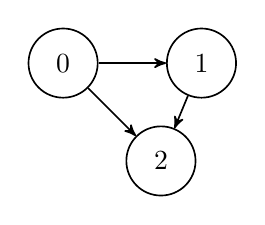
\begin{tikzpicture}[baseline=(current bounding box.center),->,>=stealth', 
	node distance=5em, semithick]
	\tikzstyle{every state}=[fill=none, draw=black, text=black]

	\node[state] (0) {0};
	\node[state] (1) [right of=0] {1};
	\node[state] (2) [below right of=0] {2};

	\path 	(0) edge node {} (1)
			(0) edge node {} (2)
			(1) edge node {} (2);
\end{tikzpicture}

	\hspace{2em}
	\begin{tabular}{l|lll}
		  & 0 & 1 & 2\\
		\hline
		0 & 0 & 0 & 0\\
		1 & 1 & 0 & 0\\
		2 & 1 & 1 & 0
	\end{tabular}
	\captionof{figure}{Example of 3-neuron network and adjacency matrix.}
	\label{fig:toyex}
\end{table}\noindent
Binary values are used throughout these toy networks: either a connection exists 
or it doesn't; either a `neuron' is spiking or it isn't. To produce spiking 
data, we create an \textit{n}-vector $\mathbb{S}$ representing the current state 
of the toy network, with random neurons already spiking based on a chosen spike 
rate. From here, the process is as in \ref{subsec:adjacency}, where $\mathbb{M}$ 
is the adjacency matrix:

\[
	\underset{n \times n}{\mathbb{M}} \times \underset{n \times 1}{\mathbb{S}^t} 
	= \underset{n \times 1}{\mathbb{S}^{t+1}}
\]
Additonally, $\mathbb{S}^{t+1}$ may have one or more neurons spike randomly, as 
determined by the spike rate of the simulation.\footnote{SEE APPENDIX} All 
values are clipped to the range $[0,1]$, to avoid double spiking.

At each step, $\mathbb{S}$ is appended to an output matrix, which is saved after 
simulation is complete. For $t$ simulation steps, the completed output has shape 
$(n \times t)$.

\subsubsection{Example Data Generation}
Consider the network defined in figure \ref{fig:toyex}. Supposing that we 
randomly spike neuron 0 at the first step, our initial state appears as such, 
where $\mathbb{O}$ is the output matrix and $\mathbb{R}$ is an \textit{n}-vector 
wherein each element has been randomly assigned 0 or 1, based on the spike rate 
of the simulation:
\[
	\mathbb{M} = \begin{bmatrix}
		0 & 0 & 0 \\
		1 & 0 & 0 \\
		1 & 1 & 0
	\end{bmatrix} \qquad
	\mathbb{S}^0 = \begin{bmatrix} 1 \\ 0 \\ 0 \end{bmatrix} \qquad
	\mathbb{O} = \begin{bmatrix} 1 \\ 0 \\ 0 \end{bmatrix}
\]
We now compute $\mathbb{S}^1$ as above:
\[
	\mathbb{S}^1 = (\mathbb{M} \times \mathbb{S}^0) + \mathbb{R} = 
		\left(\begin{bmatrix}
		0 & 0 & 0 \\
		1 & 0 & 0 \\
		1 & 1 & 0
	\end{bmatrix} \times \begin{bmatrix} 1 \\ 0 \\ 0 \end{bmatrix}\right)
	+ \begin{bmatrix} 0 \\ 1 \\ 0 \end{bmatrix}
	= \begin{bmatrix} 0 \\ 2 \\ 1 \end{bmatrix}
\]
In this case, neuron 1 was spiked randomly, but was also spiked by virtue of its 
connection from 0. Since in this simple model we only consider neurons to be 
either spiking or not, binary values, we clip the values in $\mathbb{S}^1$ to a 
maximum of 1, in order to prevent cases such as this one from causing spikes of 
greater magnitude to propagate through the network. This also prevents neurons 
from double spiking due to multiple inputs being active in the same timestep. 
Thus we have our final value for $\mathbb{S}^1$, and append it to $\mathbb{O}$.
\[
	\mathbb{S}^1 = \begin{bmatrix} 0 \\ 1 \\ 1 \end{bmatrix} \qquad
	\mathbb{O} = \begin{bmatrix}
		1 & 0\\
		0 & 1\\
		0 & 1 \end{bmatrix}
\]
If we were to repeat this process several more times, we might end up with an 
output matrix such as in figure \ref{fig:exoutput}.
\begin{figure}[H]
\[
	\mathbb{O} = \begin{bmatrix}
		1 & 0 & 1 & 0 & 0\\
		0 & 1 & 0 & 1 & 0\\
		0 & 1 & 1 & 1 & 1
	\end{bmatrix}
\]
\caption{Example output matrix for a 3-neuron network simulated for five steps.}
\label{fig:exoutput}
\end{figure}\noindent
We can clearly see the effects of neuron 2 having inputs from both other 
neurons. Practically, the number of iterations was usually set to 50.

\subsection{Generalizability}
\label{subsec:hotswap}
In most ANN implementations, feeding various data with the same label attached 
to it results in the network learning to ignore the input data and always return 
the desired label, rendering it useless. However, due to the unique structure of 
our model, this sort of overfitting is impossible (SEE SOME ARCHITECTURE 
SECTION).  Therefore, we must merely construct a suitably representative 
generator network, meaning that it contains all of the inter-neuron 
relationships we expect to see in the data we ultimately feed in to test.

\subsection{Restructuring}
The model accepts data in the form of a spike-time raster plot of dimensions $(n 
\times t)$, where \textit{n} is the number of neurons and \textit{t} is the 
number of timesteps being considered. The axes are reversed in comparison to the 
data created by the generator, and thus in the process of loading in the spike 
trains we transpose the matrices to the expected dimensionality. Additionally, 
it is not always necessary to use the full number of steps generated, depending 
on the size of the generator network in question, as well as its spike rate. In 
such a scenario, we truncate the time dimension appropriately.

For a network accepting \textit{t} timesteps of data from \textit{n} neurons, 
the data fed into the network takes the following form:
\[ \begin{bmatrix}
		x_{11} & x_{12} & \dots & x_{1n}\\
		x_{21} & x_{22} & \dots & x_{2n}\\
		\vdots & \vdots & \ddots & \vdots\\
		x_{t1} & x_{t2} & \dots & x_{tn}
	\end{bmatrix} \]
Applying this process to the data in figure \ref{fig:exoutput}, including 
truncating the time dimension to four, results in the following:
\begin{figure}[H]
	\centering
	\begin{subfigure}{.48\textwidth}
		\[
			\begin{bmatrix}
				1 & 0 & 0\\
				0 & 1 & 1\\
				1 & 0 & 1\\
				0 & 1 & 1
			\end{bmatrix}
		\]
		\caption{Transposed output matrix}
	\end{subfigure}
	\begin{subfigure}{.48\textwidth}
		\centering
		\includegraphics[width=.35\textwidth]{3outex.png}
		\caption{Graphical representation}
		\label{subfig:3outexgraph}
	\end{subfigure}
	\caption{Transposed and truncated matrix and associated visualization.}
\end{figure}\noindent
The representation of the matrix in \ref{subfig:3outexgraph} is an example of 
the method we will use to depict matrices containing real values.

\section{Architecture}
We will first describe the architecture in terms that, while accurate on the 
macro level, do not fully reflect the actual transformations occuring in the 
implemented model. We will then proceed to a mathematically representative 
version, leaving explanation of the batched version of the model to APPENDIX 
SECTION.

\subsection{Structure \& Computation Details}
\subsubsection{Dimensionality-defining Variables}
Only two values characterize the matrices and transitions involved in the model.  
They are as follows:
\begin{description}
	\item \textit{b}: The number of steps of input data the model considers in a 
		given piece of data.
	\item \textit{d}: The length of the vectors characterizing each potential 
		connection \textit{ij}. This restricts the maximum information about 
		each potential neuron pair that the model can maintain across layer 
		transitions.
\end{description}
We determined effective values for these parameters through experimentation.

Additionally, we use the number of nodes in the generator graph, \textit{n}, to 
calculate summations and averages, but the structure of our calculations is such 
that no aspects of the model are defined in terms of \textit{n}.

\subsubsection{Activation Functions}
At the end of each transition, an elementwise activation function\footnote{SEE 
THE PART OF THE BG WHERE I TALK ABOUT NN PRINCIPLES} is applied following 
completion of all computations.  For all but the final layer, that function is 
ReLU\footnote{NEEDS CITATION}, which is defined as follows:
\begin{equation}
	relu(x) = \begin{cases}
		0 & x < 0\\
		x & x \geq 0
	\end{cases}
\end{equation}

\subsection{First Transition}
To generate the first layer of the network, we inspect every pair of neurons in 
the input data. Since no pair of neurons is distinguishable from another, the 
comparison applied is the same in all cases: we apply the same convolutional 
filter to all pairs. We achieve this by concatenating the spike train of each 
neuron \textit{i} individually with every other neuron \textit{j}, then 
multiplying by a matrix $\mathbb{W}$ of dimensionality $(d \times 
2b)$.\footnote{Recall that the time dimension fed into the network is 
characterized by \textit{b}.}

$\mathbb{W}$ is trained on, and thus the comparison of each pair of spike trains 
is left up to the network. The transition appears as follows, where $\underset{b 
\times 1}{\mathbb{I}_x}$ is the input column at \textit{x}:
\[
	\mathlarger\forall i,j \mid 0 \leq i,j < n: \underset{d \times 
	1}{d_{ij}^\prime} = \underset{d \times 2b}{\mathbb{W}} \times 
	\left(\frac{\mathbb{I}_i}{\mathbb{I}_j}\right)
\]
This leaves us with $n^2$ \textit{d}-vectors, each characterizing one potential 
edge \textit{ij}.

\subsection{Convolutional Layer}
In this layer, we incorporate information from all nodes potentially adjacent to 
each edge \textit{ij}. From our previous layer, we have a matrix of shape $(d 
\times n^2)$ that we will refer to as $\mathbb{D}^{\prime}$, but it will be 
useful to keep in mind an alternate representation of that matrix, one in three 
dimensions, which we shall refer to as $\mathbb{D}_N^{\prime}$.

\begin{figure}[H]
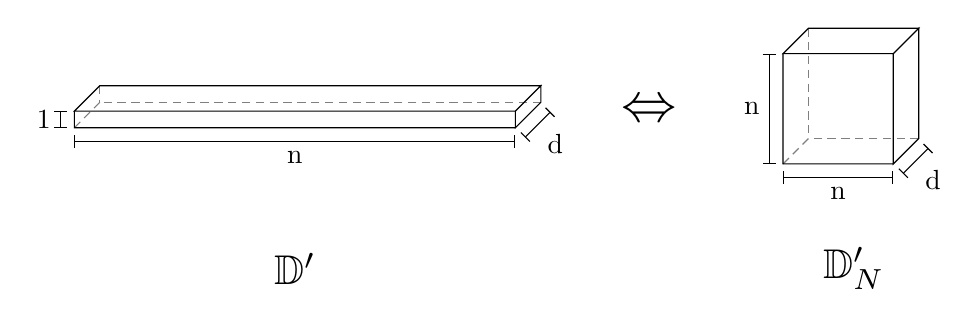
\begin{tikzpicture}
    \pgfmathsetmacro{\n}{20}
    \pgfmathsetmacro{\t}{40}
    \pgfmathsetmacro{\d}{12}
    \pgfmathsetmacro{\scale}{.07}
	\pic at (2,-1) {annotated cuboid={width=\n*4, height=3, depth=\d, xlabel=n, 
	ylabel=1, zlabel=d, scale=\scale}};
    \node at (3.7,-1) {\scalebox{2}{$\Leftrightarrow$}};
	\pic at (6.8,-.27) {annotated cuboid={width=\n, height=\n, depth=\d, 
xlabel=n, ylabel=n, zlabel=d, scale=\scale}};
	\node at (-.8, -3)  {\scalebox{1.5}{$\mathbb{D}^{\prime}$}};
	\node at (6.3, -3) {\scalebox{1.5}{$\mathbb{D}_N^{\prime}$}};
\end{tikzpicture}
\caption{Relationship between $\mathbb{D}^{\prime}$ and 
$\mathbb{D}^{\prime}_N$.}
\end{figure}\noindent
Consider some $d_{ij}^{\prime}$ in $\mathbb{D}^{\prime}_N$. Then we can say the 
following:
\begin{enumerate}
	\item $d_{ij}^{\prime}$ represents the connection from \textit{j} to 
		\textit{i} as it may or may not exist in this network, in the form of 
		\textit{d} values of indeterminate meaning
	\item $\mathlarger\forall k \mid 0 \leq k < n$, $d_{jk}^{\prime}$ represents 
		a potential input to \textit{j}
	\item $\mathlarger\forall k \mid 0 \leq k < n$, $d_{ki}^{\prime}$ represents 
		a potential output from \textit{i}
\end{enumerate}
In our determination of the presence or absence of a connection from \textit{j} 
to \textit{i}, we wish to incorporate information from these potentially 
connected nodes; i.e., these inputs and outputs represent potential neighbors in 
a graph locality sense. To achieve this, we perform the following 
computations\footnote{Actually, it's much more elegant.} for each $\underset{d 
\times 1}{d_{ij}}$:
\begin{gather}
	\begin{align}
		\label{eq:ID}
		\underset{d \times 1}{\mathbb{I}} &= \frac{1}{n} \sum_{k=0}^{n-1} 
		d_{jk}^{\prime} & \underset{d \times 1}{\mathbb{O}} &= \frac{1}{n} 
		\sum_{k=0}^{n-1} d_{ki}^{\prime}\\
		\label{eq:IDOD}
	\underset{d \times 1}{\mathbb{I_D}} &= \underset{d \times 
	d}{\mathbb{W}_{in}^\prime} \times \left(\mathbb{I} \odot 
d_{ij}^{\prime}\right) & \underset{d \times 1}{\mathbb{O_D}} &= \underset{d 
\times d}{\mathbb{W}_{out}^\prime} \times \left(\mathbb{O} \odot 
d_{ij}^{\prime}\right)
	\end{align}
	\shortintertext{\centering Here we arrive at the output,
	$d_{ij}^{\prime\prime}$:}
	d_{ij}^{\prime\prime} = \underset{d \times 2d}{\mathbb{W}_{tot}^\prime} 
	\times \left(\frac{\mathbb{I_D}}{\mathbb{O_D}}\right) \label{eq:dijO}
\end{gather}
Conceptually, in \eqref{eq:ID} we first average all potential inputs to and 
outputs from potential edge \textit{ij}. Then, we compute an entrywise product 
($\odot$) of these vectors with the vector describing the edge in question, 
$d_{ij}^{\prime}$. While we have integrated locality data into the results thus 
far, the network has not been allowed any processing over the resultant data, 
which we rectify by multiplying the input and output vectors with separate 
dimensionality-preserving $(d \times d)$ matrices. We thus arrive at 
\eqref{eq:IDOD}, with vectors $\mathbb{I_D}$ and $\mathbb{O_D}$ representing 
edge \textit{ij} with inputs and outputs, respectively, taken into 
consideration. In \eqref{eq:dijO}, we arrive at $d_{ij}^{\prime\prime}$ as it 
will be seen by the next layer of the network by multiplying a third weight 
matrix by the vertical concatenation of $\mathbb{I_D}$ and $\mathbb{O_D}$.  This 
matrix $\mathbb{W}_{tot}^\prime$, allows the network to optimize for whichever 
elements in $\mathbb{I_D}$ and $\mathbb{O_D}$ are most important in the 
prediction of \textit{ij}. The three matrices involved, 
$\mathbb{W}_{in}^\prime$, $\mathbb{W}_{out}^\prime$, and 
$\mathbb{W}_{tot}^\primt$, are trained on by the optimizer\footnote{SEE 
OPTIMIZER SECION IN TRAINING}, allowing the model to learn optimal processing 
and combinations to facilitate predictions.

Our concatenation approacb in \eqref{eq:dijO} stands in contrast to the strategy 
taken in \eqref{eq:IDOD}, where integration of the input and output data is 
forced via entrywise product computation. While we considered the same 
concatenation process for use in \eqref{eq:IDOD}, the apparent difficulty of 
integrating the calculated locality data into the prediction of \textit{ij} led 
the model to rapidly adapt its weight matrices to ignore the locality portion of 
the data.  For more discussion on this difficulty, see TRAINING SECTION.

Note again that none of the computations involved in this layer are dependent on 
\textit{n}; as the summations are averaged, the values contained in their 
resultant vectors will be of similar magnitude for any number of neurons under 
consideration. After executing this algorithm for each $d_{ij}^{\prime}$, we are 
left with another $(d \times n^2)$ output matrix, $\mathbb{D}^{\prime\prime}$.

\subsection{Final Transition}
The shift from $(d \times n^2)$ is comparatively simple, being only a 
dimensionality reduction:
\begin{equation}
	\mathlarger\forall d_{ij}^{\prime\prime} \in \mathbb{D}^{\prime\prime}:
	\underset{1 \times 1}{d_{ij}^f} = \underset{1 \times d}{\mathbb{W}^f} \times 
	\underset{d \times 1}{d_{ij}^{\prime\prime}}
\end{equation}
This leaves us with a $(1 \times n^2)$ matrix, which, following application of a 
hyperbolic tangent activation function and transposition to $(n \times n)$, we 
treat as the adjacency matrix of the generator associated with the input data.


\chapter{Training}


\section{Activation Functions}
\label{sec:activation}
\subsection{Initial \& Convolutional Layers}
At the end of each transition, an elementwise activation function is applied 
following completion of all computations, including multiplication by the 
relevant weight matrix.  For all but the final layer, that function is 
ReLU\cite{nair2010rectified}, defined in figure \ref{fig:relu}.

\begin{figure}[h]
	\centering
	\begin{minipage}{.48\textwidth}
		\begin{equation*}
			relu(x) = \begin{cases}
				0 & x < 0\\
				x & x \geq 0
			\end{cases}
		\end{equation*}
	\end{minipage}
	\begin{minipage}{.48\textwidth}
		\resizebox{\textwidth}{!}{
		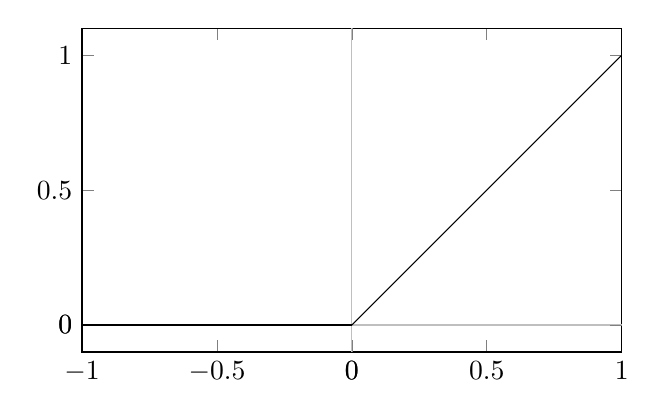
\begin{tikzpicture}
			\begin{axis}[domain=-1:1, unit vector ratio*=1 1 1,
					enlarge x limits=false, extra y ticks=0, extra x ticks=0,
					extra tick style={grid=major}]
				\addplot[color=black][domain=0:1] {x} [mark=none, smooth];
				\addplot[color=black][domain=-1:0] {0} [mark=none smooth];
			\end{axis}
		\end{tikzpicture}
		}
	\end{minipage}
	\caption{ReLU function definition and graph}
	\label{fig:relu}
\end{figure}\noindent


\subsection{Final Layer}
\label{subsec:finalactivation}
ReLU's preservation of positive values and elimination of negative values work 
in concert with the activation function of the final layer, hyperbolic tangent 
(\figref{fig:tanh}).
The clipping of negative values to 0 in previous layers of the network allows 
greater imprecision in the penultimate layer in order to predict a 0 in the 
output adjacency matrix: rather than needing to fine tune the filters to produce 
exactly 0 for nonexistent connections, the model need only drive the values for 
such neuron pairs into the negatives, and let the application of ReLU correct.  

\begin{wrapfigure}[5]{r}{.45\textwidth}
	\centering
	\vspace{-14pt}
	\resizebox{.43\textwidth}{!}{
		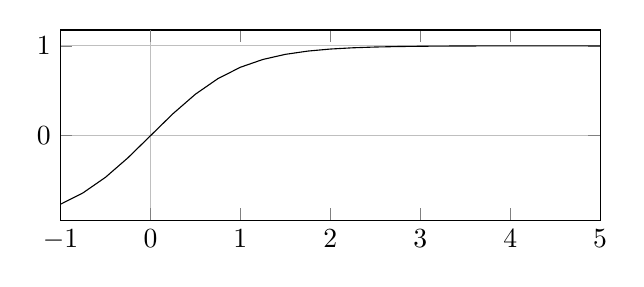
\begin{tikzpicture}
			\begin{axis}[domain=-1:5, unit vector ratio*=1 1 1,
				ytick={0,1}, enlarge x limits=false, ymajorgrids,
				xtick={-1,1,2,3,4,5},
				extra x ticks=0, extra tick style={grid=major}]
				\addplot[color=black] {tanh(x)} [mark=none, smooth];
			\end{axis}
		\end{tikzpicture}
	}
	\caption{Graph of $y=\tanh(x)$}
	\label{fig:tanh}
\end{wrapfigure}
Similarly, the final layer \textit{tanh} allows the network to drive weights for 
probable connections far into the positives, with the activation function 
ultimately mapping large values into a small range closely approaching 1.

\section{Loss \& Optimization}
\label{sec:lossandop}
In a nutshell, backpropagation via gradient descent is a method for training 
neural networks by calculating the extent to which each value in a particular 
layer is responsible for the overall network error on a single data point or 
batch, then correcting that value by an amount commensurate to its error and 
overall learning rate. This process operates from the final layer back to the 
first, hence `backpropagation'.\cite{Rumelhart}

In order to effectively descend the gradient, a network needs a function 
defining error from the desired output and an algorithm for applying gradient 
descent based on that error and a specified learning rate.

The loss function must provide useful values to the optimizer in order to allow 
effective gradient descent towards the goal, and the optimizer must adjust the 
network fast enough to converge to the target while avoiding converging to a 
suboptimal solution. As the network gets closer to an optimal state, adjusting 
at the same rate as at the start of training will almost invariably overshoot 
the desired configuration. Due to this, the optimizer must dynamically modify 
the extent to which it adjusts the network as training goes on.

\subsection{Loss Function}
% why was this so goddamn hard
\edef\myindent{\the\parindent}
\begin{minipage}{\textwidth}\setlength{\parindent}{\myindent}
\noindent We define a basic custom loss function in order to better fit the 
outputs we expect to see.

For final model output $\mathbb{O}$ and target $\mathbb{T}$, we take the sum 
squared difference, $S$, of the two vectors and the sum over $\mathbb{T}$, 
$S_T$, \eqref{eq:ssd}, and divide these two values to achieve loss 
$L$.\footnotemark
\end{minipage}
\begin{subequations}
	\centering
	\begin{align}
		S &= \sum_i \left(\mathbb{O}_i - \mathbb{T}_i \right)^2
		= \sum_i \left[\left(\mathbb{O} - \mathbb{T})_i \right)\right]^2 &
		S_T &= \sum_i \mathbb{T}_i
		\label{eq:ssd}
	\end{align}
	\begin{equation}
		L = \frac{S}{S_T}
		\label{eq:los}
	\end{equation}
	\label{eq:losscalc}
\end{subequations}

\footnotetext{Recall from \ref{subsubsec:targetdata} that the targets 
$\mathbb{T}$ given to the model are the flattend generator adjacency matrix; 
dimensionality $(1 \times n^2)$.}
Thus, rather than scale loss with the number of total possible connections 
($n^2$) as with a mean squared error, we scale our loss with the number of 
actual connections in the true adjacency matrix, keeping the loss values 
somewhat higher in the early stages of training, yet still falling to levels 
comparable to that of MSE as the model learns to predict appropriately.

%\begin{minipage}{\textwidth}
\subsubsection{Effects}
\label{subsubsec:losseffects}
\begin{wraptable}[5]{r}{.3\textwidth}
	\captionsetup{justification=centering}
	\vspace{-15pt}
	\centering
	\adjacencyT{0 & 0 & 0}{1 & 0 & 0}{1 & 1 & 0}
	\vspace{-5pt}
	\captionof{figure}{\linespread{1.2}\selectfont{}Example adjacency matrix}
	\label{fig:loss_ex}
\end{wraptable}
Consider a model analyzing data from a 3-node generator with an adjacency matrix 
as given in \figref{fig:loss_ex}, and suppose that its output is a vector 
containing two correct values and one wrong value.  Then our parameters for 
determining loss by way of \eqref{eq:losscalc} are as follows:
\begin{align*}
	\mathbb{O} &= \begin{bmatrix} 0.0 & 0.0 & 0.0 & 1.0 & 0.0 & 0.0 & 1.0 & 0.0 
			   & 1.0\end{bmatrix}\\
	\mathbb{T} &= \begin{bmatrix} 0.0 & 0.0 & 0.0 & 1.0 & 0.0 & 0.0 & 1.0 & 1.0 
				& 0.0\end{bmatrix}\\
	\left(\mathbb{O} - \mathbb{T}\right)^2 &= \begin{bmatrix} 0.0 & 0.0 & 0.0 & 
		0.0 & 0.0 & 0.0 & 0.0 & 1.0 & 1.0\end{bmatrix}\\
	S 	&= \sum_i \left(\mathbb{O}_i - \mathbb{T}_i \right)^2 = 2.0\\
	S_T &= \sum_i \mathbb{T}_i = 3.0
	\intertext{And our loss is finally determined:}
	L 	&= \frac{S}{S_T} = \frac{2.0}{3.0} = .\overline{6}
\end{align*}
%\end{minipage}
Thus, our loss function `punishes' the network equally for false positives and 
false negatives: due to the squared difference, a 1 where there should be a 0 
adds the same loss as a 0 where there should be a one. This is perhaps not the 
ideal method; see \ref{subsec:lossdisc}. The value produced for each 
input/target pair is then passed to the optimizer.

\subsection{Optimizer Function}
\label{subsec:optimizer}
We used the Adam optimizer as provided by 
TensorFlow\cite{tensorflow2015-whitepaper}, providing different initial learning 
rates per dataset. Those values were arrived at via experimentation. After 
initializing the optimizer, it is passed the loss at each step and performs 
gradient descent on the trainable matrices.

Adam adjusts its learning rate as time goes on, according to the following 
equation, where $\beta_n^t$ indicates exponentiation by $t$ and $lr$ denotes 
learning rate:
\begin{figure}[h]
	\begin{minipage}[b]{.38\textwidth}
		\centering
		\begin{gather}
			\nonumber
			\beta_1 = 0.9\\
			\nonumber
			\beta_2 = 0.999\\
			\nonumber
			lr_t = lr_{init} \times \frac{\sqrt{1-\beta_2^t}}{1-\beta_1^t}
		\end{gather}
	\end{minipage}
	\hfill
	\begin{minipage}{.6\textwidth}
		\centering
		\resizebox{\textwidth}{!}{
			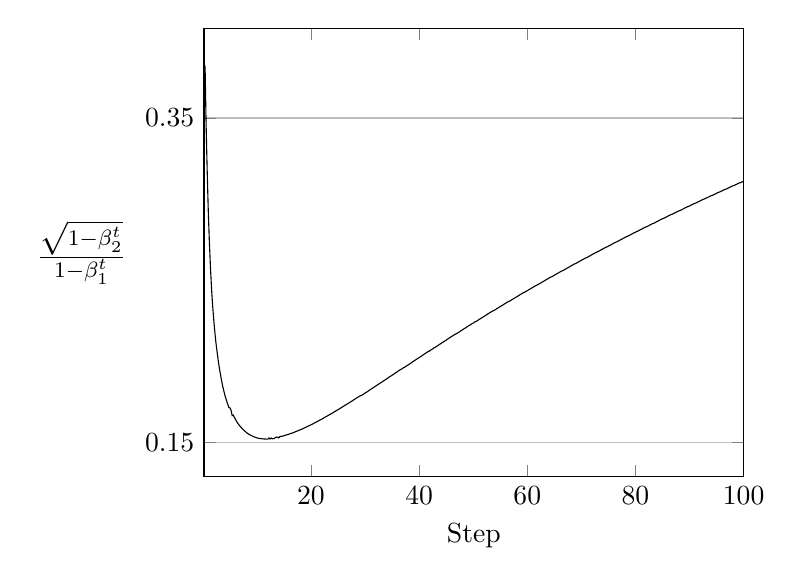
\begin{tikzpicture}
			\begin{axis}[domain=.01:100, ytick={0,.15,.35}, samples=500,
				ylabel=$\frac{\sqrt{1-\beta_2^t}}{1-\beta_1^t}$,
				ylabel style={rotate=-90, font=\large},
					enlarge x limits=false, ymajorgrids, extra x ticks=0,
					extra tick style={grid=major}, xlabel=Step]
					\addplot[color=black] {sqrt(1-.999^x)/(1-.9^x)} [mark=none, 
			smooth];
			\end{axis}
		\end{tikzpicture}
		}
		\captionof{figure}{Adam decay function over 100 steps. Converges 
			asymptotically to 1.}
	\end{minipage}
\end{figure}


\section{Matrices}
\subsection{Initialization}
Initially, we seeded our matrices with random values from a normal distribution 
of standard deviation 1.0 and mean 0, using the TensorFlow implementation of 
\texttt{tf.random\_normal(<dimensions>)}. Due, however, to the cumulative nature 
of our matrix operations (in the locality layer, for instance, there are three 
separate multiplications (\ref{subsubsec:matconvlayer})), we found that the 
values of the outputs were so high or low as to render the model somewhat random 
in its convergence, or lack thereof.

We found that by reducing the standard deviation of our distributions to 0.25, 
we can ensure that most, if not all, training runs of our model converge. If 
raised higher, models trained on complex generator networks may consistently 
fail to converge, and a lower value tends to lead to convergence on non-optimal 
solutions, such as prediciting all zeroes. 

\subsection{Locality Layer Operations}
\label{subsec:localops}
As discussed in \ref{subsubsec:locality}, a different method for integrating 
inputs and outputs to a given edge was originally considered. If $\mathbb{I}$ is 
the average input vector for some edge $d_{ij}$, and $\mathbb{O}$ is the average 
output vector, then the original operations went as follows:
\begin{subequations}
\begin{align}
	\underset{d \times 1}{\mathbb{I_D}} &= \underset{d \times 
	2d}{\mathbb{W}_{in}^\prime} \times 
	\left(\frac{\mathbb{I}}{d_{ij}^\prime}\right) &
	\underset{d \times 1}{\mathbb{O_D}} &= \underset{d \times 
		2d}{\mathbb{W}_{out}^\prime} \times 
		\left(\frac{d_{ij}^\prime}{\mathbb{O}}\right)
\end{align}
\begin{equation}
		d_{ij}^{\prime\prime} = \mathbb{I_D} + \mathbb{O_D}
\end{equation}
\end{subequations}
This was suboptimal for a variety of reasons. The addition of the two vectors in 
the final step implied that both inputs and outputs were of exactly equal value 
in determining the existence of an edge, and even further that, for any index 
into those two vectors, the values at that index would be usefully comparable in 
some way.

Beyond this, the integration of locality data in this format seemed to require 
careful tuning, and gradient descent did not work well with this setup.  
Specifically, at an initial network state, the first layer has not been 
optimized to provide useful data targeted at the second layer summations that 
produce $\mathbb{I}$ and $\mathbb{O}$. However, the only reason for the network 
to trend towards this type of data shaping in the first layer would be an 
observed decrease in loss. While doubtless possible, it seems a more attractive 
(loss optimizing) option appears: zero the left side of 
$\mathbb{W}_{in}^\prime$, and the right of $\mathbb{W}_{out}^\prime$. As the 
noisy locality data is removed from the system, the loss decreases, and 
eventually the network arrives at a somewhat remarkable state: the halves of the 
weight matrices that remain in use converge to the same values, operating as 
they are on the same data.

For these reasons, we opted for the implementation described in 
\ref{subsubsec:locality}, in which we force the integration of locality data 
into the model's calculations via entrywise multiplication, and provide an 
optimizable matrix for combining input and output data, allowing the network to 
learn which parts are most important.

\section{Hyperparameter Optimization}
\subsection{Batch Size}
`Batching' refers to the process of assembling a set of items from the training 
data and passing them through the network in parallel, then optimizing over the 
resulting losses simultaneously. This greatly speeds computation speed by 
removing the costly optimization operation from each step. We found that 32 
units per batch was an effective number, offering high training speeds with 
relatively stable loss curves.


%! TEX root = /home/hsartoris/sproj/writeup/main.tex
\graphicspath{ {resources/models/3neurEx/} {resources/models/3neurEx/weights/} } 

\chapter{Results}
\label{results}
\section{Overfitting}
\label{sec:overfitting}
\setlength{\columnsep}{20pt}
\begin{wraptable}[8]{r}{.4\textwidth}
	\captionsetup{justification=centering}
	\vspace{-20pt}
	\begin{tabular}{lr}
		b (timesteps) & 8\\
		d& 5\\
		Batch size& 32\\
		Training steps& 20000\\
		Learning rate& .0005\\
		Training samples& 18000\\
		Validation samples& 4500
	\end{tabular}
	\vspace{-5pt}
	\captionof{figure}{\linespread{1.2}\selectfont{}Training parameters for 
		null hypothesis network}
	\label{fig:nullparams}
\end{wraptable}
As discussed in \ref{subsec:hotswap} and \ref{subsec:n-independence}, the unique 
structure of our model prevents it from overfitting to a particular generator 
topology, allowing us to create a single generator containing connections 
representative of the types of data we expect to analyze with the trained model.
We demonstrate this aspect of our architecture in two test cases: by training 
models on an empty dataset paired with one adjacency matrix throughout, and 
training with a random dataset paired with that same adjacency matrix.

\subsection{Empty Data}
We ran a combined 100 training sessions of the benchmark model and our 
convolutional model, with parameters as defined in \figref{fig:nullparams}, on a 
dataset whose inputs contained only zeroes and whose target was the adjacency 
matrix in \figref{fig:2simplex+adjacency}. For both models, exactly two losses 
and corresponding outputs repeatedly occurred (\figref{fig:empty_loss}), with 
the models demonstrating a total inability to memorize the target data.

\begin{figure}[h]
	\centering
	\begin{subfigure}{.45\textwidth}
		\centering
		\begin{tabular}{cccc}
				   &  0 &  1 &  2\\\cline{2-4}
			\mc{0} & .3 & .3 & .3\\
			\mc{1} & .3 & .3 & .3\\
			\mc{2} & .3 & .3 & .3
		\end{tabular}
		\caption{loss: $0.\overline{6}$}
	\end{subfigure}
	\begin{subfigure}{.45\textwidth}
		\centering
		\begin{tabular}{llll}
			  & 0 & 1 & 2\\\cline{2-4}
			\mc{0} & 0 & 0 & 0\\
			\mc{1} & 0 & 0 & 0\\
			\mc{2} & 0 & 0 & 0
		\end{tabular}
		\caption{loss: 1.0}
	\end{subfigure}
	\caption{Predictions and losses when training on an empty dataset}
	\label{fig:empty_loss}
\end{figure}

\section{3-neuron generator}
\label{results_3neur}
We first consider a generator network consisting of three nodes connected as in 
\figref{fig:2simplex+adjacency}. All weights are binary, and a spike rate of 
.25 was used.\footnote{SEE APPENDIX	for information on spike rates} 

\begin{table}[h]
	\centering
	\captionsetup{margin=5em}
	
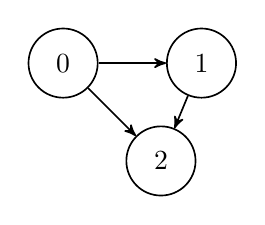
\begin{tikzpicture}[baseline=(current bounding box.center),->,>=stealth', 
	node distance=5em, semithick]
	\tikzstyle{every state}=[fill=none, draw=black, text=black]

	\node[state] (0) {0};
	\node[state] (1) [right of=0] {1};
	\node[state] (2) [below right of=0] {2};

	\path 	(0) edge node {} (1)
			(0) edge node {} (2)
			(1) edge node {} (2);
\end{tikzpicture}

	\hspace{2em}
	\begin{tabular}{llll}
		& 0 & 1 & 2\\\cline{2-4}
		\mc{0} & 0 & 0 & 0\\
		\mc{1} & 1 & 0 & 0\\
		\mc{2} & 1 & 1 & 0
	\end{tabular}
	\captionof{figure}{Network structure and adjacency matrix of the generator.  
	(Reproduced from Figure \ref{fig:toyex})}
	\label{fig:2simplex+adjacency}
\end{table}\noindent
Reconstructing this simplified graph allows us to demonstrate that our 
convolutional approach is capable of reconstruction.  Furthermore, the small 
generator size requires few timesteps and a small interlayer featurespace; i.e., 
$b,d<10$.  This results in a relatively simple set of transitions, allowing us 
to explore and understand the inner workings of the network.

\subsection{Example Model}
\label{subsec:3neurex}
The following data are pulled from a model trained on data produced by the 
generator in \figref{fig:2simplex+adjacency}. Figure 
\ref{fig:3neur_loss+params} demonstrates the model's loss over time. In this 
example, \textit{b} and \textit{d} were pushed down in order to allow for better 
comprehension of the internal mechanics; the loss tends to converge more 
effectively and evenly given more computation power.
%! TEX root = /home/hsartoris/sproj/writeup/main.tex
\begin{table}[h]
	\centering
	\begin{minipage}{.48\textwidth}
	\resizebox{\textwidth}{!}{
		\begin{tikzpicture}
			\begin{semilogyaxis} [xlabel=Step, ylabel=Loss, scaled x 
				ticks=false,
				axis lines*=left,
				xtick={1,25000,50000},
				legend cell align=left,
				legend style={ anchor=north east},
				extra y ticks={.0497}, extra y tick style={grid=major},
				%ytick={1}, 
				yticklabel style={	/pgf/number format/precision=2,
									/pgf/number format/fixed}]
				\addplot [color=black] table [x=Step, y=Loss, col sep=comma, 
			mark=none, smooth] {../resources/models/9neur/minFinalConv_90};
				\addlegendentry{Locality-based}
				\addplot [color=black, dashed] table [x=Step, y=Loss, col 
			sep=comma, mark=none, smooth] 
			{../resources/models/9neur/minFinalDumb_72};
				\addlegendentry{Benchmark}
			\end{semilogyaxis}
		\end{tikzpicture}
	}
	\end{minipage}
	\hfill
	\begin{minipage}{.48\textwidth}
		\centering
		\begin{tabular}{lr}
			\textit{b} (timesteps) & 30\\
			\textit{d}& 40\\
			Batch size& 32\\
			Learning rate& .001\\
			Training samples& 36000\\
			Validation samples& 9000\\
		\end{tabular}
	\end{minipage}
	\captionof{figure}{Loss \& parameters for model trained on data from 
		generator given in \figref{fig:10neur}}
	\label{fig:9neur_loss+params}
\end{table}


\subsubsection{Trained Network Operation}
Here, we examine in brief the internal operation of the trained model over a 
single input. For a complete look through the procedure of reconstruction for 
this network, please see APPENDIX.
\begin{figure}[h]
	\centering
	\begin{subfigure}{.15\textwidth}
		\centering
		\includegraphics[width=.75\textwidth]{9/input.png}
		\caption{Input}
		\label{subfig:3neur_in}
	\end{subfigure}
	\hspace{1em}
	\begin{subfigure}{.3\textwidth}
		\includegraphics[width=\textwidth]{9/out0.png}
		\caption{Data after first transform}
	\end{subfigure}
	\hspace{1em}
	\begin{subfigure}{.3\textwidth}
		\includegraphics[width=\textwidth]{9/out1.png}
		\caption{Data after convolutional layer}
		\label{subfig:3neur_out1}
	\end{subfigure}
	\caption{Path of data through network, up to final transform}
	\label{fig:3neur_input}
\end{figure}

The last transformation of the network involves a matrix multiplication of the 
final layer weights\footnote{see appendix} with the data in 
\ref{subfig:3neur_out1}. This produces the adjacency matrix found in figure 
\ref{fig:3neur_pred}.

\begin{table}[h]
	\centering
	\adjacencyT{.02 & .03 & .01}{.99 & .01 & -.01}{1.0 & 1.0 & .02}
	\captionof{figure}{Output for input data in \figref{subfig:3neur_in}}
	\label{fig:3neur_pred}
\end{table}

\section{Applicability Beyond Training Data}
As described in \ref{subsec:hotswap}, the fact that our model is trained on data 
produced by only one generator is of little consequence; due to its structure, 
the only information it can learn is relational; i.e., per-neuron-pair. Consider 
the following examples, in which data was produced from several generator 
networks and fed into the model described in \ref{results_3neur}:


TODO: add examples of input and output data to 3.2.1 and 3.2.2.

\subsection{Inverted Network}
\begin{table}[h]
	\centering
	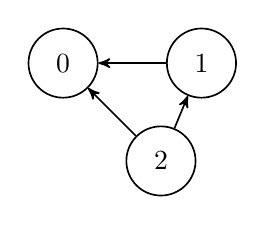
\begin{tikzpicture}[baseline=(current bounding box.center),->,>=stealth', 
	node distance=5em, semithick]
	\tikzstyle{every state}=[fill=none, draw=black, text=black]

		\node[state] (0) {0};
		\node[state] (1) [right of=0] {1};
		\node[state] (2) [below right of=0] {2};
	
		\path 	(2) edge node {} (1)
				(2) edge node {} (0)
				(1) edge node {} (0);
	\end{tikzpicture}
	\hspace{2em}
	\begin{tabular}{l|lll}
		  & 0 & 1 & 2\\
		\hline
		0 & 0 & 1 & 1\\
		1 & 0 & 0 & 1\\
		2 & 0 & 0 & 0
	\end{tabular}
	\captionof{figure}{Inverted version of \figref{fig:2simplex+adjacency}}
	\label{fig:2simplexVar1}
\end{table}
\noindent Despite being a complete inversion of the generator used to train the 
model in \ref{results_3neur}, reconstruction of this network is simple.

\begin{table}[h]
	\centering
	\begin{minipage}{.1\textwidth}
		\includegraphics[width=\textwidth]{var1/input.png}
	\end{minipage}
	\hspace{2em}
	{\scalebox{2}{$\Rightarrow$}}
	\hspace{2em}
	\begin{tabular}{l|lll}
		  & 0 & 1 & 2\\
		\hline
		0 & .01 & 1.00 & 1.00\\
		1 & .01 & .02 & 1.00\\
		2 & 0 & .02 & .01
	\end{tabular}
\end{table}

\subsection{Cyclical Network}
\label{subsec:cyclical}
\begin{table}[h]
	\centering
	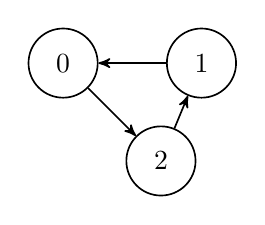
\begin{tikzpicture}[baseline=(current bounding box.center),->,>=stealth', 
	node distance=5em, semithick]
	\tikzstyle{every state}=[fill=none, draw=black, text=black]

		\node[state] (0) {0};
		\node[state] (1) [right of=0] {1};
		\node[state] (2) [below right of=0] {2};
	
		\path 	(2) edge node {} (1)
				(0) edge node {} (2)
				(1) edge node {} (0);
	\end{tikzpicture}
	\hspace{2em}
	\begin{tabular}{l|lll}
		  & 0 & 1 & 2\\
		\hline
		0 & 0 & 1 & 0\\
		1 & 0 & 0 & 1\\
		2 & 1 & 0 & 0
	\end{tabular}
	\captionof{figure}{Cyclical 3-neuron network}
	\label{fig:2simplexVar2}
\end{table}

\noindent For a cyclical network, the situation is not quite so simple. Due to 
the perpetual propagation of spikes through the generator, additional random 
spiking can cause the input data to become an impenetrable mess. Tempering the 
spike rate to 0.05 produces workable data, but the results are neither so clean 
nor
consistent as for terminating networks.  




%! TEX root = /home/hsartoris/sproj/writeup/main.tex
\chapter{Discussion}
As described in \ref{sec:localitybroken}, in all cases tested, models equipped 
with our locality layer tended to stay very close to the benchmark models in 
loss, with a slight tendency towards higher loss. This tendency is explained by 
the simple presence of more values to optimize over. More to the point, we must 
return to the motivation behind incorporating locality into network 
reconstruction: we hope that our model will learn to recognize recurrent local 
structures in biological networks, and use that information to judge individual 
connection probability in the context of its neighbors. Two potential factors in 
our model's failure to manifest this behavior are apparent: data used, and 
specific locality algorithm design.

\section{Data}
An important part of analyzing the performance of our locality layer is to 
understand what we are looking for. In the cases tested, the locality-enabled 
model was not able to outstrip the benchmark model in terms of loss or 
predictive accuracy, but this likely speaks more to the type of data being used 
to train the networks than to the relative efficacy of either architecture. If 
three matrix multiplications are sufficient to reconstruct the structure of a 
network, there is little need for a model to involve abstract concepts like 
locality, and, even if forced to do so, it's not clear that having such concepts 
available would contribute to more effective reconstruction. The ideal test 
dataset, then, would be one on which the benchmark model does not converge to an 
accurate prediction, allowing us to train a locality-enabled model and get some 
idea of how much useful information is actually added. Here, we outline some 
directions we could go in data generation.

\subsection{Complex Neurons}
As it stands, every generator we used to produce data consisted of binary 
connections and created binary outputs. There are clearly more accurate methods 
of simulating biological neural network activity, such as implementing 
Izhikevich neurons\footnote{Cite}, or going as far as generating data with
NEST\footnote{citation}. However, while more complex neurons would probably 
encourage the model to look to locality for information, this alone would not 
suffice.

\subsection{Larger, Structured Networks}
A model being able to leverage its access to locality data to locate 2-simplices 
will not encounter any particular benefit from this ability if the generators it 
is tasked with reconstructing contain at most one such structure. Indeed, 
preliminary results suggest that a large gap opens between models considering 
locality and those not when the training data is generated from a large 
($n\approx50$) network seeded with recurring motifs. On such a dataset, the 
benchmark model cannot get below .5 loss, while the locality-enabled model hits 
.35 easily.

\section{Improvements to Locality Processing}

\subsection{Layering}
There may need to be more initial layers to provide useful data to the Locality 
layers.  As it stands, the model structure requires that the first layer both 
compare the activities of neuron pairs and format the resulting data in such a 
manner that the locality-based layer can usefully include it in determining node 
existence.  Adding at least one intermediary processing layer might allow the 
network to format the data going in to the locality layer in a more useful way.  
Merits further testing.

\subsection{Loss}
\label{subsec:lossdisc}
As described in \ref{subsubsec:losseffects}, our custom loss function equally 
weights false positives and false negatives. Consider these cases:

\begin{enumerate}
	\item Output 0.3; target 1.0: adds $(0.3-1.0)^2=0.49$ to the loss
	\item Output 0.7; target 0.0: adds $(0.7-0.0)^2=0.49$ to the loss
\end{enumerate}
Despite the equivalent loss contributions, the latter case is the less correct 
of the two: while guessing a weak connection where there is a strong one is not 
ideal, it is preferable to guessing a strong connection where there is none.  
Thus our loss function might be modified to more strongly disincentive false 
positives.

\section{Potential Applications/Further Development}

In the process of creating this network, we implemented a pure-numpy version, 
which can run on matrices created by a model trained in TensorFlow. This would, 
along with the portability of our model, allow for training and then 
distributing ready-to-run reconstruction models, without the need for user 
experience with GPUs, machine learning, or any of the like.


%! TEX root = /home/hsartoris/sproj/writeup/main.tex
\begin{appendices}
	\chapter{Appendix}
	%\chapter{Model}
	\section{Batched Architecture Calculations}
	\label{asec:batched}
	In order to allow processing of many pieces of data at once, the matrix 
	model defined in \ref{subsec:matmodel} was adapted to a batched format.  
	Given input matrices of shape $(b \times n)$, the actual input to the model 
	is now of shape $(batchSize \times b \times n)$. As previously discussed, 
	iteration across lists or dimensions is not a computationally efficient 
	option. Therefore we use \texttt{tf.einsum}, an implementation of Einstein 
	Sums. This allows, for example, the multiplication of two matrices, one of 
	dimension $(i \times j \times k)$, and the other of dimension $(h \times 
	j)$. An appropriate function call might appear as
	\texttt{tf.einsum(`hj,ijk->ihk', mat2, mat1)}. The result is equivalent to 
	the iterative multiplication of the $(h \times j)$ matrix across all 
	\textit{i}, without the computational overhead of CPU involvement. Every 
	matrix multiplication in our model is implemented using this functionality.

\end{appendices}




\end{document}
